\section{Árvore Rubro Negra}
\label{sec:rubro}

Como uma alternativa mais relaxada à Arvore AVL, a Arvore Rubro Negra surgiu do trabalho "A Dichromatic Framework for Balanced Trees"\ de Leonidas J. e Robert Sedgewick, e a escolha das cores rubro e negra foram influenciados pela disponibilidade de canetas dessa cor na época e qualidade de impressão.

Para atender a necessidade de se auto balancear, a Rubro-Negra assume algumas regras e características:

\begin{enumerate}
	\item Todo nó é vermelho (rubro) ou preto (negro).
	\item O nó raiz é preto.
	\item Toda folha (\texttt{Nil}) é preto.
	\item Se um nó é vermelho, seus dois filhos são pretos.
	\item Cada caminho da raiz até um nó \texttt{Nil} tem a mesma quantidade de nós pretos.
\end{enumerate}

\begin{figure}[!ht]
	\centering
	\adjustbox{max width=\textwidth}{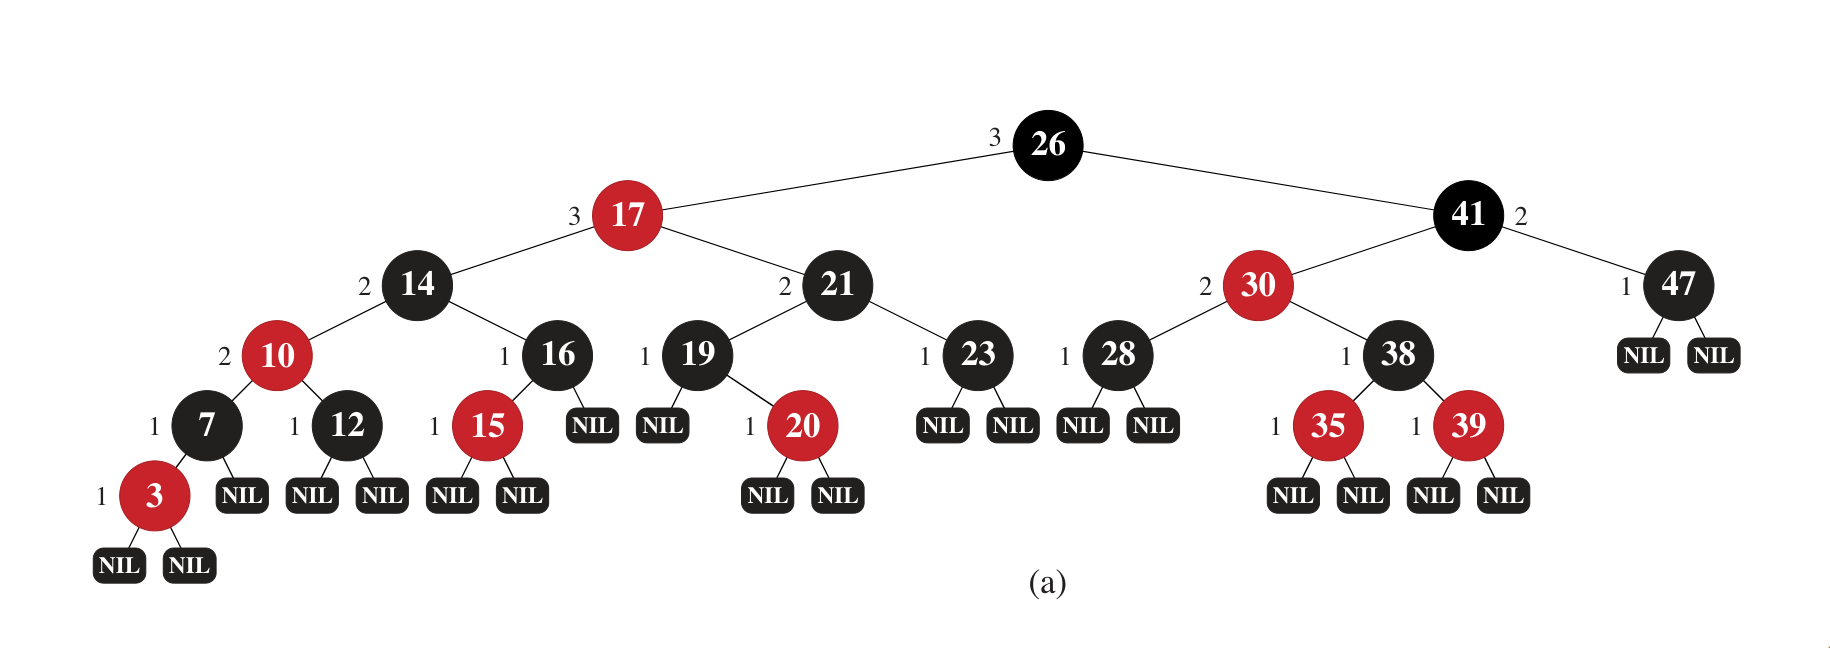
\includegraphics{figures/rubro-negra/example.png}}
	\caption{Exemplo de Árvore Rubro Negra}
	\label{fig:rubro_example}
\end{figure}
\FloatBarrier

% TODO: Adicionar nota de rodapé indicando origem da imagem 

Devida sua natureza, uma árvore rubro negra de $n$ elementos tem \textit{profundidade} de ao máximo $2\lfloor\log (n + 1)\rfloor$, garantindo que as operações de \textrm{I\textsc{nserção}}, \textrm{B\textsc{usca}}, \textrm{R\textsc{emoção}} tenham complexidade $O(\log n)$ no pior caso.

\subsection{Implementação}

Para sua implementação, usaremos a linguagem de programação Haskell, assumindo a seguinte estrutura.

\begin{lstlisting}[language=haskell]
data RedBlackTree a
  = Node
      { color :: Color
      , left :: RedBlackTree a
      , key :: a
      , right :: RedBlackTree a
      }
  | Nil
\end{lstlisting}

Um elemento do tipo \texttt{RedBlackTree a}, onde \texttt{a} é genérico pode ser a função \texttt{Node} que recebendo quatro argumentos, a cor (\texttt{color}), a árvore esquerda (\texttt{left}), o valor dentro do nó (\texttt{key}) e a árvore direita (\texttt{right}) se torna uma \texttt{RedBlackTree a}, ou pode ser diretamente o valor \texttt{Nil}, que implicitamente tem cor preta.

Neste documento implementaremos a \textrm{I\textsc{nserção}} e \textrm{R\textsc{emoção}}, visto que as implementações da \textrm{B\textsc{usca}} e \textrm{R\textsc{otação}} são análogas a árvore AVL e binária.

\subsubsection{Inserção}

Inicialmente, o algoritmo será similar a inserção na Árvore binária convencional, mas uma vez inserido o valor em algum nó, precisamos decidir qual será sua cor e garantir que as regras da Rubro-negra seja atendida.

Em relação a cor, escolheremos a cor vermelha, pois minimiza a quantidade de violações das características, caso seja a raiz, simplesmente pintaremos esse nó de preto. Teremos então:

\begin{lstlisting}[language=haskell]
insert :: (Ord a) => a -> RedBlackTree a -> RedBlackTree a
insert value tree = makeRootBlack $ insert' value tree
\end{lstlisting}
\FloatBarrier

Naturalmente, os valores que uma Rubro-negra precisa armazenar devem ser ordenáveis (restrição imposta por \texttt{Ord a}), ademais, no primeiro momento, usaremos duas funções auxiliares, a \texttt{makeRootBlack} e \texttt{insert'}.

Começando pela mais simples, a \texttt{makeRootBlack} será simplesmente:

\begin{lstlisting}[language=haskell]
makeRootBlack :: RedBlackTree a -> RedBlackTree a
makeRootBlack (Node _ left key right) = Node Black left key right
\end{lstlisting}
\FloatBarrier

Na \texttt{insert'} podemos prosseguir, assim como uma inserção tradicional em uma árvore binária, apenas com algumas ressalvas.

\begin{lstlisting}[language=haskell]
insert' value Nil = Node Red Nil value Nil  -- inicialmente como vermelho
insert' value (Node color left key right)                      
  | value < key = balance color (insert' value left) key right  
  | value > key = balance color left key (insert' value right) 
  | otherwise = Node color left key right                      
\end{lstlisting}
\FloatBarrier

Usaremos mais uma função auxiliar chamada \texttt{balance}, que terá a mesma tipagem do construtor \texttt{Node} e será responsável por corrigir as possíveis violações locais causadas pela inserção do novo nó vermelho. Vamos analisar tais violações, ao tentar insertar um valor:

\begin{itemize}
	\item \textbf{Violação Esquerda-Esquerda:} Dois vermelhos na sub-árvore esquerda. \\
	      Uma vez chegando no caso base e inserindo o valor \texttt{x}, essa violação ocorrerá da seguinte forma:
	      \begin{figure}[!ht]
		      \centering
		      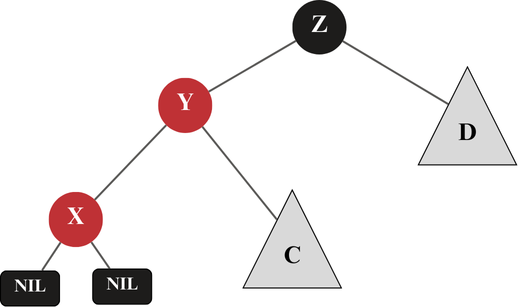
\includegraphics[scale=0.5]{figures/rubro-negra/left-left-insertion.png}
		      \caption{}
	      \end{figure}
	      \FloatBarrier
	      E para resolver localmente essa violação, rotacionamos e alteramos as cores da árvore da seguinte forma:
	      \begin{figure}[!ht]
		      \centering
		      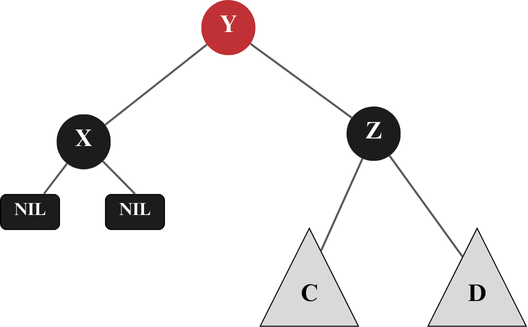
\includegraphics[scale=0.5]{figures/rubro-negra/left-left-base-solution.png}
		      \caption{}
	      \end{figure}
	      \FloatBarrier
	      Entretanto, depois de balancear essa sub-árvore, a raiz vermelha pode ser filho de algum outro nó vermelho na árvore maior. Mas, como a \texttt{balance} é chamada em cada etapa do \texttt{insert'}, logo ela vai continuar corrigindo as violações nas sub-árvores até a topo da árvore. Então generalizamos esse caso:
	      \begin{figure}[!ht]
		      \centering
		      \begin{minipage}{0.4\textwidth}
			      \centering
			      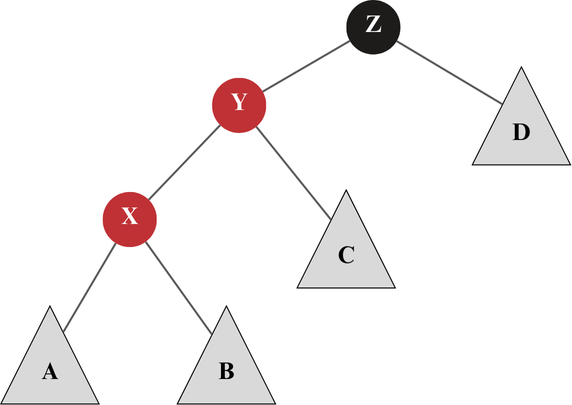
\includegraphics[scale=0.42]{figures/rubro-negra/left-left.png}
			      \caption{}
			      \label{fig:left-left}
		      \end{minipage}%
		      \hspace{1em}
		      \textbf{$\Longrightarrow$}
		      \hspace{1em}
		      \begin{minipage}{0.4\textwidth}
			      \centering
			      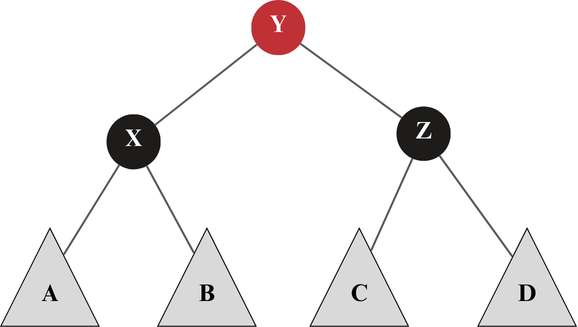
\includegraphics[scale=0.42]{figures/rubro-negra/left-left-solution.png}
			      \caption{}
			      \label{fig:left-left-solution}
		      \end{minipage}
	      \end{figure}
	      \FloatBarrier
	\item \textbf{Violação Esquerda-Direita:} Dois vermelhos, um no filho esquerdo e outro no filho-filho direito.
	      \begin{figure}[!ht]
		      \centering
		      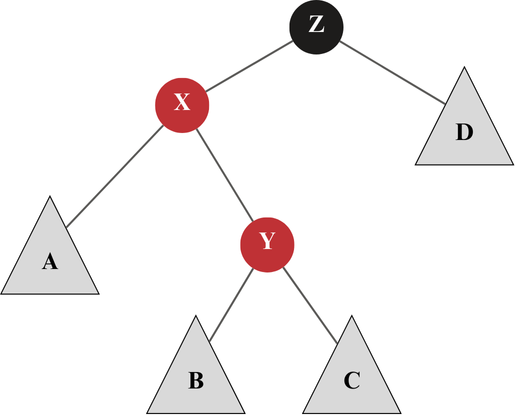
\includegraphics[scale=0.5]{figures/rubro-negra/left-right.png}
		      \caption{}
	      \end{figure}
	      \FloatBarrier
	      Para resolver essa violação, também vamos reconfigurar como foi feito na Figura \ref{fig:left-left-solution}, assim como todas as restantes.
	\item \textbf{Violação Direita-Direita:} Dois vermelhos, na sub-árvore direita.
	      \begin{figure}[!ht]
		      \centering
		      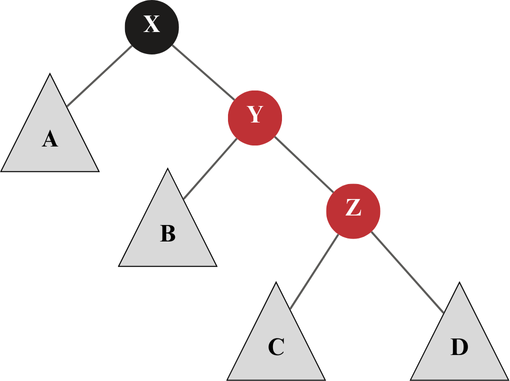
\includegraphics[scale=0.5]{figures/rubro-negra/right-right.png}
		      \caption{}
	      \end{figure}
	      \FloatBarrier
	\item \textbf{Violação Direita-Esquerda} Dois vermelhos, um no filho direito e outro no filho-filho esquerdo.
	      \begin{figure}[!ht]
		      \centering
		      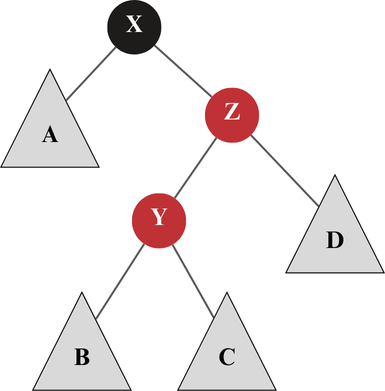
\includegraphics[scale=0.5]{figures/rubro-negra/right-left.png}
		      \caption{}
	      \end{figure}
	      \FloatBarrier
\end{itemize}

\noindent
Uma vez estabelecidos os casos a, implementação desse algoritmo se torna bem mais simples do que em versões iterativas, visto que todos os casos produzem o mesmo resultado.

\begin{lstlisting}[language=haskell]
-- Esquerda-Esquerda
balance Black (Node Red (Node Red at x bt) y ct) z dt =
  Node Red (Node Black at x bt) y (Node Black ct z dt)
-- Esquerda-Direita
balance Black (Node Red at x (Node Red bt y ct)) z dt =
  Node Red (Node Black at x bt) y (Node Black ct z dt)
-- Direita-Direita
balance Black at x (Node Red (Node Red bt y ct) z dt) =
  Node Red (Node Black at x bt) y (Node Black ct z dt)
-- Direita-Esquerda
balance Black at x (Node Red bt y (Node Red ct z dt)) =
  Node Red (Node Black at x bt) y (Node Black ct z dt)
-- Padrao
balance color left key right = Node color left key right
\end{lstlisting}
\FloatBarrier

% TODO:
% - Exemplo de teste
% - Revisão
